\section{Analysis}

\begin{frame}{Analysis: Effect of Exploration}
\begin{figure}
    \centering
    \begin{subfigure}{\textwidth}
        \centering
        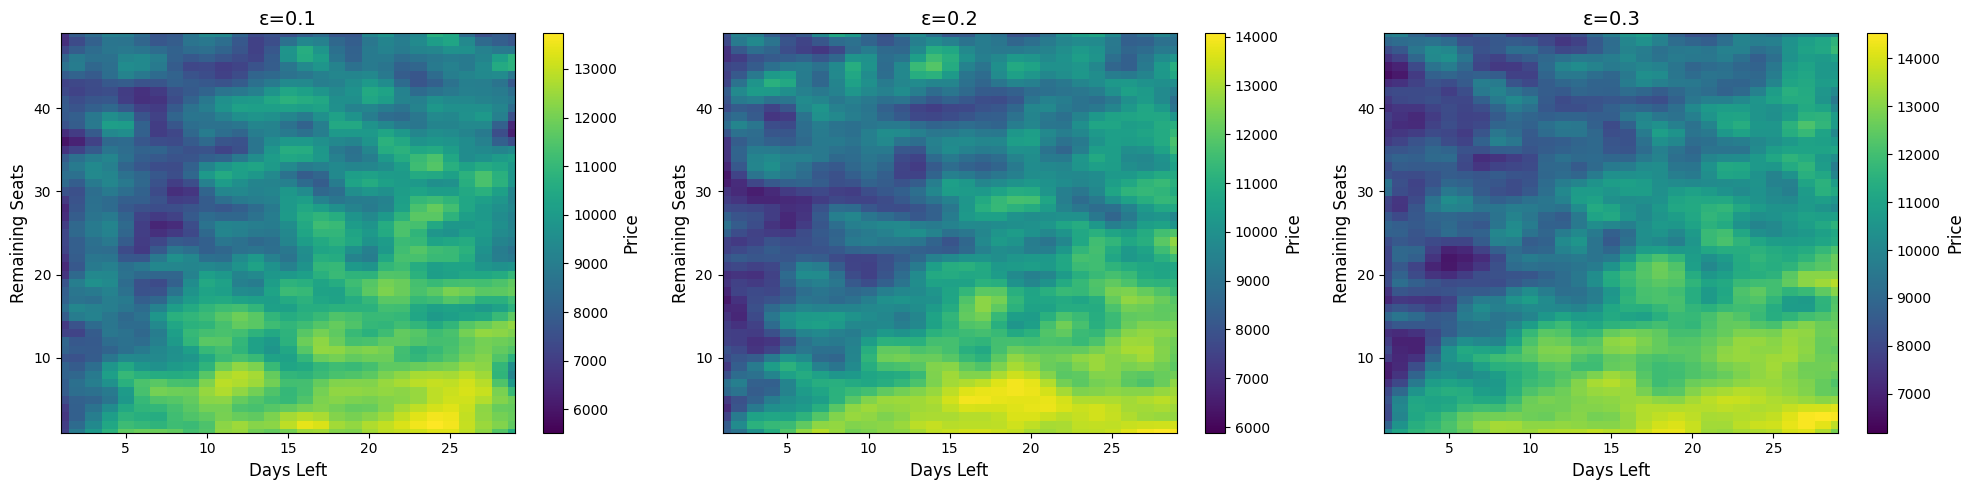
\includegraphics[width=\textwidth]{epsilon_policy.png}
        \caption{Learned Policy}
    \end{subfigure}
    \begin{subfigure}{\textwidth}
        \centering
        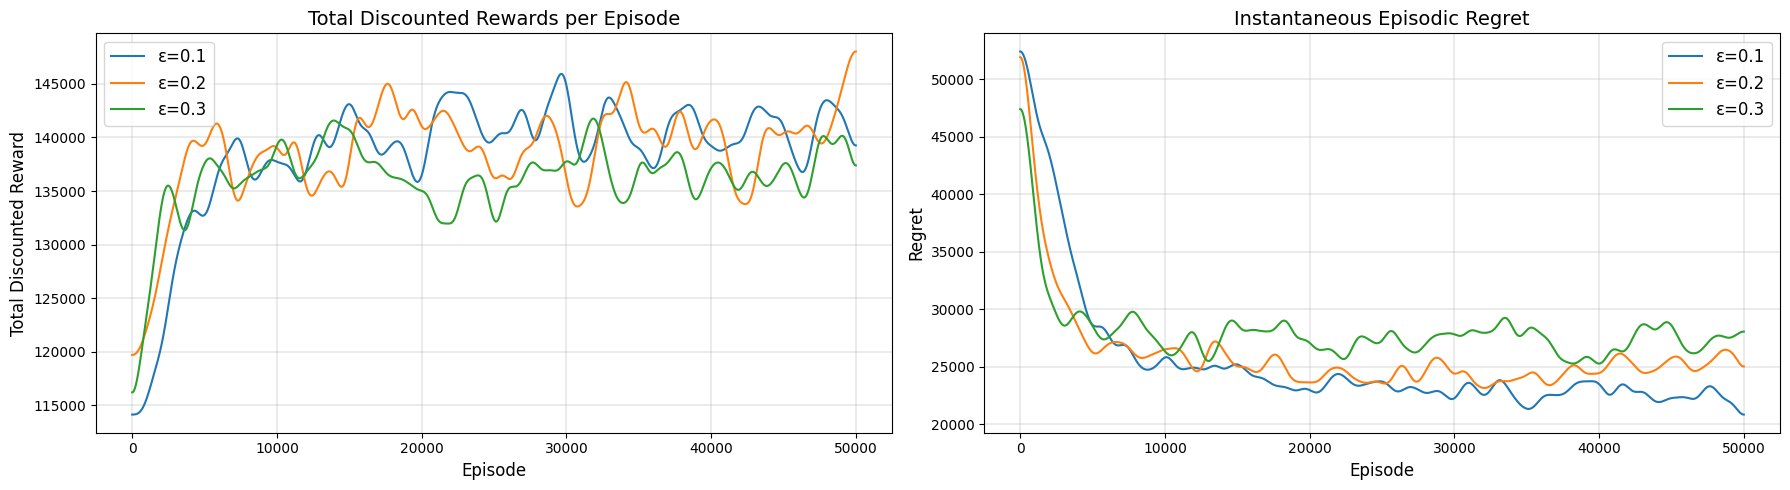
\includegraphics[width=0.9\textwidth]{epsilon_metrics.png}
        \caption{Episodic Rewards and Regrets}
    \end{subfigure}
    \caption{Q-Learning at different levels of $\epsilon-$greedy Exploration}
\end{figure}
\end{frame}

\begin{frame}{Analysis: Effect of Trace Decay}
\begin{figure}
    \centering
    \begin{subfigure}{\textwidth}
        \centering
        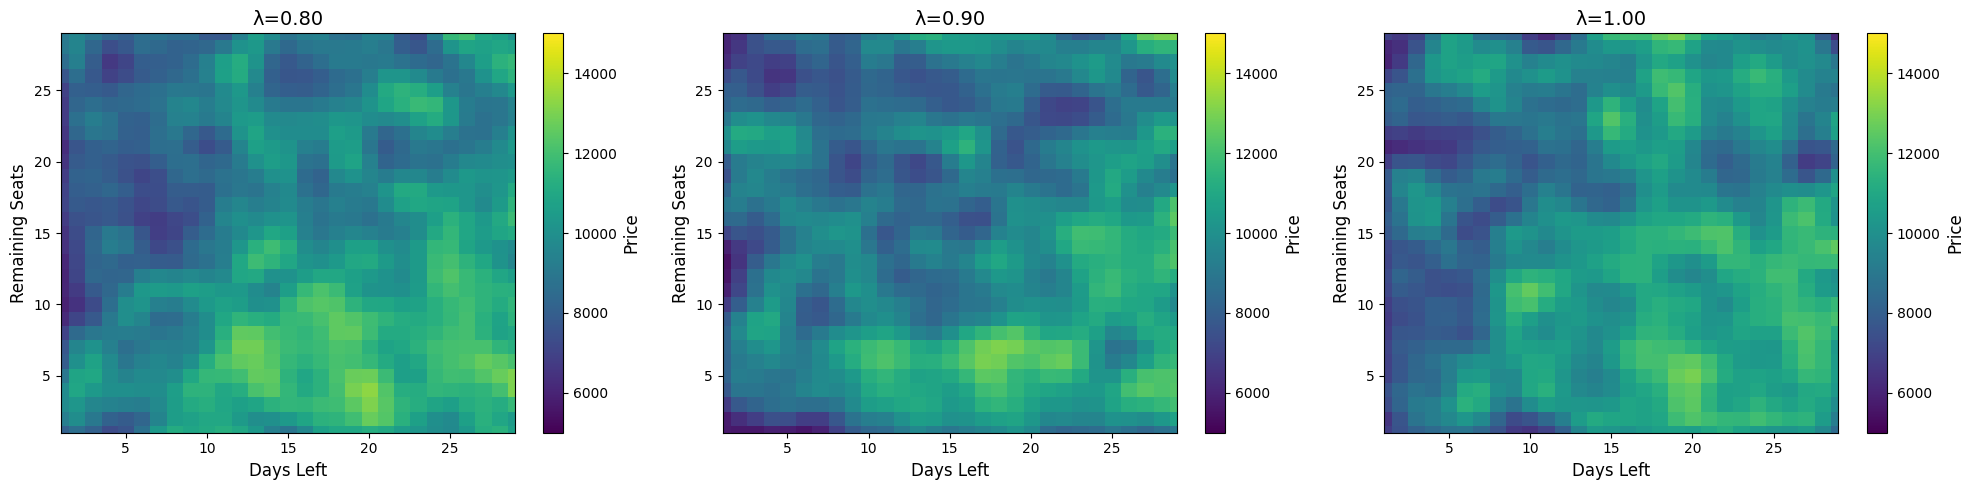
\includegraphics[width=\textwidth]{lambda_policy.png}
        \caption{Learned Policy}
    \end{subfigure}
    \begin{subfigure}{\textwidth}
        \centering
        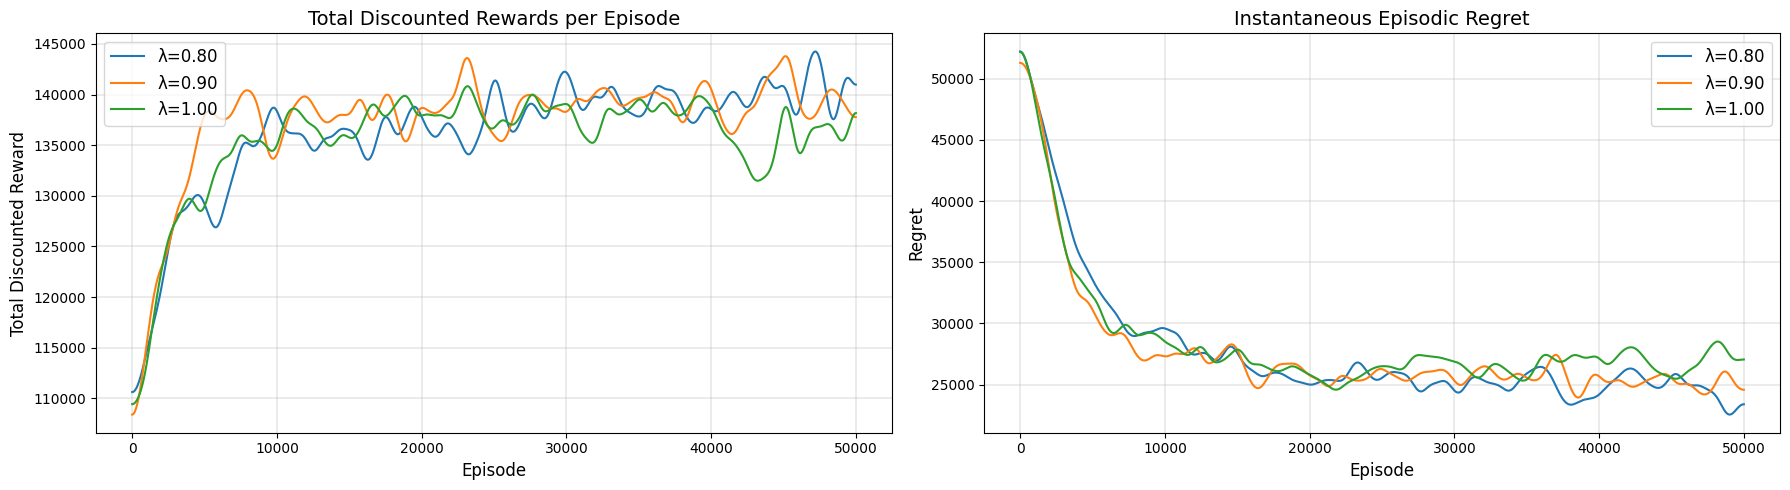
\includegraphics[width=0.9\textwidth]{lambda_metrics.png}
        \caption{Episodic Rewards and Regrets}
    \end{subfigure}
    \caption{SARSA($\lambda$) at different levels of Trace Decay}
\end{figure}
\end{frame}

\begin{frame}{Conclusion}
\begin{itemize}
    \setlength\itemsep{1.5em}
    \item Learned policies tend to clear inventory faster than optimal policy, when nearing the end of booking window.
    \item Learned policies lacked similarity in close neighbourhood, likely due to the possibility of covering up for initial choices later.
    \item Convergence rate was similar in Q-Learning and SARSA($\lambda$). However, Q-Learning got closer to the optimal policy and acquired less regret.
    \item Q-Learning tends to overestimate the value function initially, slowly stabilising as the number of episodes increases.
    \item The effect of exploration and trace decay parameter is not very prominent in the value function, but tends to influence the policy slightly.
\end{itemize}
\end{frame}
